%% ICML-format, reader-friendly rewrite of paper_draft/main.tex.
%% Uses the ICML 2026 style as a stand-in until the ICML 2027 style is released.
%% Every number in this file comes from ../results/ (see make_icml_tables.py,
%% make_icml_figures.py and check_numbers.py).
\documentclass{article}

\usepackage{microtype}
\usepackage{graphicx}
\usepackage{booktabs}
\usepackage{hyperref}
\usepackage{xurl}
\newcommand{\theHalgorithm}{\arabic{algorithm}}
\usepackage{icml2026}

\usepackage{amsmath,amssymb,mathtools,amsthm,bm}
\usepackage{algorithm}
\usepackage{algorithmic}
\usepackage{tikz}
\usetikzlibrary{arrows.meta,positioning,calc,shapes.geometric}
\usepackage[capitalize,noabbrev]{cleveref}
\usepackage{xspace}

\theoremstyle{plain}
\newtheorem{proposition}{Proposition}

\graphicspath{{figures/}{../results/paper_assets/}}

\newcommand{\method}{One-sided $\Delta$-Physics\xspace}
\newcommand{\dphys}{$\Delta$-Physics\xspace}
\newcommand{\std}[1]{\,{\scriptsize$\pm$#1}}
\newcommand{\RelL}{\mathrm{RelL2}}
\newcommand{\PSRE}{\mathrm{PSRE}}
\newcommand{\F}{\mathcal{F}}

\icmltitlerunning{Change the Physics, Not the Network}

\begin{document}

\twocolumn[
  \icmltitle{Change the Physics, Not the Network:\\
    Zero-Shot Viscosity Transfer for Frozen Neural PDE Solvers}

  \icmlsetsymbol{equal}{*}
  \begin{icmlauthorlist}
    \icmlauthor{Anonymous Authors}{anon}
  \end{icmlauthorlist}
  \icmlaffiliation{anon}{Anonymous Institution}
  \icmlcorrespondingauthor{Anonymous Authors}{anon@example.com}
  \icmlkeywords{neural operators, PDE surrogates, parameter shift, zero-shot transfer, test-time adaptation}
  \vskip 0.3in
]

\printAffiliationsAndNotice{}

\begin{abstract}
A neural PDE solver trained at one viscosity becomes inaccurate when it is asked about a fluid with a different viscosity, and the usual fix, simulating and training at the new value, is exactly the cost the solver was meant to avoid.
We show that for a shift toward \emph{higher} viscosity no new data or training is needed.
Viscosity enters the equations only through a linear diffusion term whose one-step effect is known in closed form, so we keep the trained network frozen and add the difference between the target and training diffusion propagators, computed with one FFT per step.
We call this \method, as it is switched off for lower viscosities, where in our tests the same correction degraded long rollouts; it adds no parameters, keeps one network evaluation per step, and returns exactly the original model at the training viscosity.
At twice the training viscosity, it reduces the 50-step rollout error of a frozen F-FNO on 2D Navier--Stokes by 22\% and of a frozen FNO on 1D viscous Burgers by 92\%. It also matches an iterative zero-shot baseline to within 1\% while using about 9$\times$ fewer network evaluations.
\end{abstract}

%% ============================================================
\section{Introduction}
\label{sec:intro}

Suppose you have trained a neural time-stepper, a Fourier neural operator that advances a two-dimensional flow by one time step, on simulations at viscosity $\nu_0$.
A colleague now asks how the same flow would evolve if the fluid were twice as viscous.
The usual answers are to simulate the flow at $2\nu_0$ and fine-tune, or to have trained on a range of viscosities from the start \citep{gupta2023multiscale,kirchmeyer2022coda,koupai2024geps}.
Both require simulations at the new parameter, which is the expensive step the surrogate was supposed to remove.
Running the frozen network unchanged is not an answer either: its rollouts keep too much fine-scale energy (\cref{fig:teaser}a), and the error grows with the size of the viscosity shift (\cref{fig:teaser}b,c).

\begin{figure*}[t]
  \centering
  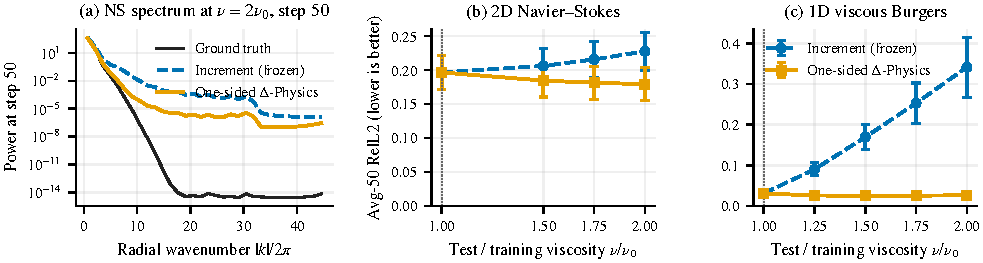
\includegraphics[width=\textwidth]{fig1_teaser.pdf}
  \vspace{-1.6em}
  \caption{\textbf{The problem and the fix.}
  A network trained only at viscosity $\nu_0$ is rolled out at a higher viscosity $\nu$ without retraining.
  \textbf{(a)}~2D Navier--Stokes at $\nu=2\nu_0$ after 50 steps: the frozen network (blue, dashed) keeps far too much power at high wavenumbers, because it still damps fine scales at the rate it learned for $\nu_0$. Adding the known extra damping (orange) removes much of this excess; mean over 24 test trajectories pooled across three seeds.
  \textbf{(b, c)}~Average error over a 50-step rollout as the test viscosity moves away from the training value. The frozen network degrades with the shift; with \method the error stops growing. Error bars: sample s.d.\ over three seeds.}
  \label{fig:teaser}
\end{figure*}

Our starting point is that viscosity does not change the physics in an arbitrary way.
It enters the governing equation through one linear term, $\nu\Delta u$, and the effect of that term over one time step is known exactly: in Fourier space it multiplies each mode $k$ by $e^{-\nu|k|^2\Delta t}$.
A network trained at $\nu_0$ has already learned to apply the $\nu_0$ version of this damping.
So instead of asking the network to learn how its output should depend on $\nu$, we keep it frozen and add only the \emph{difference} between the $\nu$ and $\nu_0$ damping, a closed-form correction that costs one FFT per step.
If the dynamics were purely diffusive and the network perfect, this correction would turn the $\nu_0$ solver into an exact $\nu$ solver.

In our experiments the correction is useful in only one direction.
Adding damping (for $\nu>\nu_0$) is benign.
For $\nu<\nu_0$ the same formula adds energy back at fine scales. It stays bounded, and with a perfect network it would still be exact, but with a real network it improves the first step and then ruins long rollouts.
We therefore apply the correction only when $\nu>\nu_0$ and call the method \method.

We test it on two PDEs and two backbones: 2D forced Navier--Stokes with a factorized FNO (F-FNO; \citealp{tran2023ffno}) and 1D viscous Burgers with an FNO \citep{li2021fno}.
At $\nu=2\nu_0$, the 50-step error falls by 22\% on Navier--Stokes and 92\% on Burgers, and on Burgers the corrected error stays essentially flat as the viscosity doubles (\cref{fig:teaser}c).
The gain grows with both the viscosity shift and the rollout horizon, and spectral diagnostics show it comes from removing the damping mismatch.
An iterative zero-shot alternative inspired by equation recasting \citep{cheng2026recast} reaches nearly the same accuracy with about 9$\times$ more network evaluations.
A model trained with data at every test viscosity is still far more accurate, so \method is a tool for when such data are not available, not a replacement for them.

\textbf{Contributions.}
\begin{itemize}
  \setlength\itemsep{1pt}
  \item A training-free way to transfer a frozen neural time-stepper to a higher viscosity: add the closed-form difference of two diffusion propagators after each network step (\cref{sec:method}). It has no parameters, recovers the original model exactly at $\nu_0$, and is exact for pure diffusion. A local error analysis shows what it misses: the interaction between the extra diffusion and the nonlinear dynamics (\cref{prop:local}).
  \item An ablation showing that, in our setting, the correction should be applied only toward higher viscosity, and an account of what the sign of the correction does and does not imply (\cref{sec:one_sided,sec:why_one_sided}).
  \item Evidence on two PDEs and two neural-operator backbones that the gain grows with the shift and the horizon and targets the spectral mismatch, together with an accuracy--cost comparison against an iterative zero-shot baseline and multi-viscosity supervision (\cref{sec:results}).
\end{itemize}
The method covers one parameter, viscosity, that enters through a known linear dissipative term, and only shifts toward stronger dissipation; \cref{sec:limitations} lists the limits of our evidence.

%% ============================================================
\section{Setting}
\label{sec:setting}

\textbf{PDEs with a known dissipative part.}
We consider dissipative PDEs that split into a linear part controlled by the parameter and everything else,
\begin{equation}
  \partial_t u = \nu \mathcal{L} u + \mathcal{N}(u),
  \label{eq:pde}
\end{equation}
where $\mathcal{L}$ is a known, negative semidefinite linear operator and $\mathcal{N}$ collects nonlinear terms and forcing.
For both PDEs studied here $\mathcal{L}=\Delta$ on a periodic domain: viscous Burgers, $\partial_t u + u\,\partial_x u = \nu\,\partial_{xx}u$, and incompressible Navier--Stokes in vorticity form, $\partial_t\omega + \bm v\cdot\nabla\omega = \nu\Delta\omega + f$.

\textbf{Neural time-stepper.}
A neural operator $F_\theta$ is trained on trajectories at a single reference viscosity $\nu_0$ to predict the change of the state over a step $\Delta t$:
\begin{equation}
  \Phi_\theta(u_t) = u_t + F_\theta(u_t) \approx u_{t+\Delta t}.
  \label{eq:stepper}
\end{equation}
At test time it is rolled out autoregressively, feeding each prediction back as the next input.
We refer to this frozen predictor as \emph{Increment} in tables and figures.

\textbf{Zero-shot viscosity transfer.}
After training, $\theta$ is frozen. We are given a new viscosity $\nu$, which is known, but \emph{no} trajectories at $\nu$.
The goal is a better rollout at $\nu$ without new data, without updating $\theta$, and without adding test-time optimisation.

%% ============================================================
\section{\method}
\label{sec:method}

\subsection{Intuition: the pure-diffusion case}
\label{sec:intuition}

Over one step of length $\Delta t$, the linear part of \cref{eq:pde} alone evolves the state by the \emph{diffusion propagator}
\begin{equation}
  S_\nu = \exp(\nu\Delta t\,\mathcal{L}),\qquad
  \widehat{S_\nu u}(k) = e^{-\nu|k|^2\Delta t}\,\hat u(k),
  \label{eq:semigroup}
\end{equation}
where $\hat u=\F[u]$ and $k$ is the physical wavenumber ($k_j=2\pi n_j/\ell_j$ on a periodic box of side $\ell_j$).
Each Fourier mode decays at its own rate, and fine scales decay fastest.

Take the simplest case, $\mathcal{N}=0$, and suppose the network has learned the $\nu_0$ dynamics perfectly, so that $\Phi_\theta=S_{\nu_0}$.
Adding the difference of propagators gives
\begin{equation}
  \Phi_\theta u + (S_\nu - S_{\nu_0})u = S_{\nu_0}u + (S_\nu - S_{\nu_0})u = S_\nu u,
  \label{eq:exact_linear}
\end{equation}
which is exactly the solver for the new viscosity.
Note that we add the \emph{difference}, not $S_\nu$ itself: the frozen network already contains the $\nu_0$ damping, and adding the full target damping would count it twice.

To make the size of the correction concrete: at $\nu=2\nu_0$ in our Navier--Stokes setting ($\nu_0=10^{-3}$, $\Delta t=0.05$), the extra per-step damping $e^{-(\nu-\nu_0)|k|^2\Delta t}$ is $0.998$ for the lowest mode ($|k|=2\pi$) but $0.13$ for mode $32$ along an axis.
The frozen network leaves out a small, scale-dependent amount of damping at every step, and the shortfall compounds over a rollout.
This is the excess fine-scale power in \cref{fig:teaser}a.

\subsection{The correction}

For the full nonlinear PDE we apply the same idea at every step of the rollout:
\begin{equation}
  \hat u_{t+\Delta t} = \underbrace{\hat u_t + F_\theta(\hat u_t)}_{\text{frozen network}} \;+\;
  \underbrace{\mathbb{1}[\nu>\nu_0]\,(S_\nu - S_{\nu_0})\,\hat u_t}_{\text{known physics}},
  \label{eq:delta_physics}
\end{equation}
where, for the periodic Laplacian,
\begin{equation}
  (S_\nu - S_{\nu_0})u = \F^{-1}\!\Big[\big(e^{-\nu|k|^2\Delta t} - e^{-\nu_0|k|^2\Delta t}\big)\,\hat u(k)\Big].
  \label{eq:fourier}
\end{equation}
\Cref{fig:method} and \cref{alg:method} show the whole procedure.
The name \dphys refers to this difference in known physics between the target and reference viscosities.
The correction does not try to model how viscosity changes the nonlinear dynamics $\mathcal{N}$; it fixes only the part of the shift that is known analytically.

\begin{figure}[t]
\centering
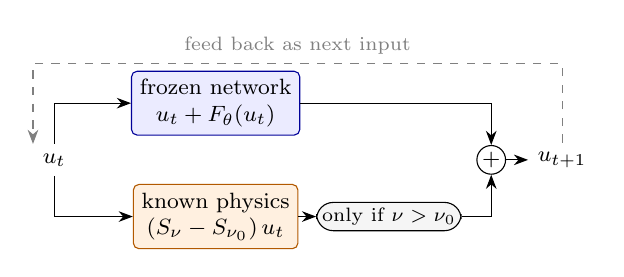
\begin{tikzpicture}[
  font=\footnotesize, >={Stealth[length=1.8mm]},
  box/.style={draw, rounded corners=2pt, align=center, minimum height=8mm, inner sep=3pt},
  net/.style={box, fill=blue!8, draw=blue!60!black},
  phys/.style={box, fill=orange!12, draw=orange!70!black},
  gate/.style={draw, rounded corners=6pt, inner sep=2pt, fill=gray!8, font=\scriptsize}]
  \node (u) at (0,0) {$u_t$};
  \node[net]  (nn) at (2.05, 0.72) {frozen network\\$u_t+F_\theta(u_t)$};
  \node[phys] (ph) at (2.05,-0.72) {known physics\\$(S_\nu-S_{\nu_0})\,u_t$};
  \node[gate] (g)  at (4.25,-0.72) {only if $\nu>\nu_0$};
  \node[circle, draw, inner sep=0.6pt] (plus) at (5.55,0) {$+$};
  \node (out) at (6.45,0) {$u_{t+1}$};
  \draw[->] (u.north) |- (nn.west);
  \draw[->] (u.south) |- (ph.west);
  \draw[->] (nn.east) -| (plus.north);
  \draw[->] (ph.east) -- (g.west);
  \draw[->] (g.east) -| (plus.south);
  \draw[->] (plus) -- (out);
  \draw[->, dashed, gray] (out.north) -- ++(0,1.0) -| node[pos=0.25, above, font=\scriptsize, text=gray] {feed back as next input} (u.north west);
\end{tikzpicture}
\caption{\textbf{One rollout step of \method.} The network is unchanged and evaluated once. The known physics branch adds the extra damping that the new viscosity requires (one FFT and one element-wise multiply). For $\nu\le\nu_0$ the branch is switched off and the step equals the original model.}
\label{fig:method}
\end{figure}

\begin{algorithm}[t]
  \caption{Rollout with \method}
  \label{alg:method}
  \begin{algorithmic}[1]
    \STATE {\bfseries Input:} frozen $F_\theta$ trained at $\nu_0$; target $\nu$; step $\Delta t$; initial state $u_0$; horizon $T$
    \STATE $m(k) \gets e^{-\nu|k|^2\Delta t} - e^{-\nu_0|k|^2\Delta t}$ \hfill $\triangleright$ precomputed once
    \FOR{$t=0$ {\bfseries to} $T-1$}
      \STATE $u_{t+1} \gets u_t + F_\theta(u_t)$ \hfill $\triangleright$ one network call
      \IF{$\nu>\nu_0$}
        \STATE $u_{t+1} \gets u_{t+1} + \F^{-1}[\,m \odot \F[u_t]\,]$ \hfill $\triangleright$ $O(N\log N)$
      \ENDIF
    \ENDFOR
    \STATE {\bfseries return} $u_1,\dots,u_T$
  \end{algorithmic}
\end{algorithm}

\subsection{Why only one side}
\label{sec:one_sided}

For $\nu>\nu_0$ every Fourier multiplier in \cref{eq:fourier} is negative: the correction only removes energy, and removes more of it at fine scales.
For $\nu<\nu_0$ the sign flips and the correction \emph{adds} energy, mostly at fine scales.
This is not the ill-posed backward heat equation: the multipliers then lie between 0 and 1, so the correction stays bounded, and with a perfect network the corrected step would still be the exact solver at $\nu$ (\cref{prop:properties}(ii) holds in both directions without the indicator).
What changes is that the correction now adds back a fraction of the current state's fine-scale content, including whatever errors the network has accumulated there.
Whether this is harmful depends on the network, so we settled it empirically: in \cref{sec:why_one_sided} the two-sided correction improves the first step below $\nu_0$ and then degrades long rollouts.
Hence the indicator in \cref{eq:delta_physics}: below $\nu_0$ we fall back to the unchanged network.
The one-sided rule is an empirical policy for dissipative transfer, not a proven requirement.

\subsection{Properties}
\label{sec:properties}

\begin{proposition}[Safe by construction]
\label{prop:properties}
(i) At $\nu=\nu_0$ the corrected stepper equals $\Phi_\theta$ exactly.
(ii) If $\mathcal{N}=0$ and $\Phi_\theta=S_{\nu_0}$, then for every $\nu>\nu_0$ the corrected stepper equals $S_\nu$ (without the indicator, also for $\nu<\nu_0$).
(iii) If $\mathcal{L}$ is self-adjoint and negative semidefinite and $\nu\ge\nu_0$, then $\langle u,(S_\nu-S_{\nu_0})u\rangle\le 0$ for all $u$, so the correction never adds energy.
\end{proposition}
The proofs are one line each (\cref{app:proofs}).
Property (iii) concerns the correction alone.
It is \emph{not} a stability guarantee for the full learned rollout, which also depends on the network.

\textbf{What the correction misses.}
Adding the propagator difference is one way to attach the known physics to the network; composing them, as in operator splitting \citep{strang1968construction,mclachlan2002splitting}, is another.
With $h=\Delta t$ and $B=(\nu-\nu_0)\mathcal{L}$, compare the additive step $\Phi_{\mathrm{add}}=\Phi_\theta+(S_\nu-S_{\nu_0})$ with the Lie step $\Phi_{\mathrm{Lie}}=e^{hB}\Phi_\theta$ and the Strang step $\Phi_{\mathrm{Str}}=e^{hB/2}\,\Phi_\theta\,e^{hB/2}$.
\begin{proposition}[Local error with an exact reference step]
\label{prop:local}
For the spatially discretised system with smooth $\mathcal{N}$, let $\varphi^h_\nu$ be the exact flow at viscosity $\nu$ and suppose $\Phi_\theta=\varphi^h_{\nu_0}$. Then, at fixed resolution,
\begin{align*}
\varphi^h_\nu-\Phi_{\mathrm{add}} &= \tfrac{h^2}{2}\,(\mathcal{N}'B+B\mathcal{N})+O(h^3),\\
\varphi^h_\nu-\Phi_{\mathrm{Lie}} &= \tfrac{h^2}{2}\,(\mathcal{N}'B-B\mathcal{N})+O(h^3),\\
\varphi^h_\nu-\Phi_{\mathrm{Str}} &= O(h^3),
\end{align*}
where $(\mathcal{N}'B\pm B\mathcal{N})(u)=\mathcal{N}'(u)Bu\pm B\mathcal{N}(u)$.
\end{proposition}
The proof is a Taylor expansion (\cref{app:proofs}); a numerical check on a small nonlinear system is included with the code.
The additive correction is exact for the linear part but leaves the whole interaction between the extra diffusion and the nonlinear dynamics uncorrected at second order; in the Lie step the two interaction terms partly cancel, and the Strang step removes them at this order.
These statements assume an exact reference step.
A trained network is not exact, and the pre-damping in the Strang step feeds it states it never saw in training, so which form works best for a \emph{frozen} network is an empirical question that we have not yet answered (\cref{sec:limitations}).

\textbf{Cost.} Training is unchanged and uses only $\nu_0$ data.
At test time each step costs one network evaluation plus an FFT pair, $O(N\log N)$ for $N$ grid points.
There are no new parameters, no target trajectories, and no fixed-point iterations.

%% ============================================================
\section{Experimental setup}
\label{sec:setup}

\textbf{PDEs and data.}
\emph{2D Navier--Stokes}: forced vorticity equation on the periodic unit square at $64\times64$, forcing $f=0.1[\sin 2\pi(x{+}y)+\cos 2\pi(x{-}y)]$, $\nu_0=10^{-3}$, network step $\Delta t=0.05$.
\emph{1D viscous Burgers}: periodic unit interval, 64 points, $\nu_0=10^{-2}$, $\Delta t=0.02$.
Ground truth comes from a pseudo-spectral RK4 solver with dealiasing.
For each seed we train on 24 trajectories of 20 transitions (480 input--output pairs) at $\nu_0$ only, and test on 8 trajectories per viscosity, with 50-step free-running rollouts.
For a given seed the test initial conditions are identical across viscosities, so differences between viscosities are not confounded by the starting state.

\textbf{Models.}
Navier--Stokes uses an F-FNO \citep{tran2023ffno} (width 16, 8 modes, 8 layers; 28,370 parameters); Burgers uses an FNO \citep{li2021fno} (width 32, 16 modes, 4 layers).
Both predict normalised increments and are trained for 15 epochs with Adam.
All main results use three independently trained seeds; we report mean\,$\pm$\,sample standard deviation.
\Cref{app:setup} gives every remaining setting.

\textbf{Metrics.}
Relative $L^2$ error at selected steps (\emph{Step-$n$ RelL2}) and averaged over the 50-step rollout (\emph{Avg-50 RelL2}).
Because the correction acts on the spectrum, we also report the power-spectrum relative error $\PSRE=\|P_{\hat u}-P_u\|_2/\|P_u\|_2$ with $P_u(k)=|\F[u](k)|^2$, averaged over the rollout (\emph{Avg-50 PSRE}).

\textbf{Comparisons.}
(1)~The \emph{frozen network} (Increment), which is our direct baseline because \method only adds a term to it.
(2)~A \emph{Recast-style} zero-shot baseline, our adaptation of equation recasting \citep{cheng2026mdpnop,cheng2026recast} to a time-stepper: it feeds the viscosity difference through the network, re-evaluating the network at every iteration until a fixed point is reached (\cref{app:recast}). It is not an official implementation of either method.
(3)~A \emph{conditioned F-FNO} trained on five viscosities that include every test value: an upper reference that uses the target data we assume are unavailable.

%% ============================================================
\section{Results}
\label{sec:results}

\subsection{Does the correction help, and does the help grow with the shift?}
\label{sec:ns}

\begin{figure*}[t]
  \centering
  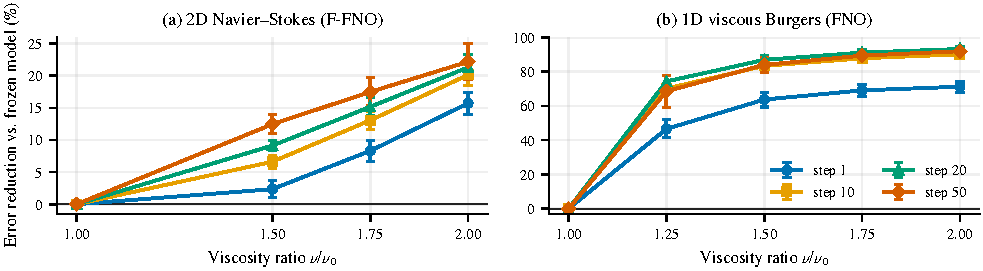
\includegraphics[width=\textwidth]{fig3_horizon_curves.pdf}
  \vspace{-1.6em}
  \caption{\textbf{The gain grows with the viscosity shift and with the rollout horizon.} Relative reduction in RelL2 error of \method over the same frozen network, at rollout steps 1--50. Zero at $\nu=\nu_0$ by construction. Mean\,$\pm$\,s.d.\ over three seeds. The two panels use different vertical scales.}
  \label{fig:horizon}
\end{figure*}

\begin{table*}[t]
\caption{\textbf{Original models: the additive correction on the frozen network.} Error after 50 autoregressive steps
(Step-50 RelL2) and average spectral error over the rollout (Avg-50 PSRE); lower is better.
Mean\,$\pm$\,sample standard deviation over three independently trained seeds; bold marks the better
of the two columns. At $\nu=\nu_0$ the two methods are identical by construction. Navier--Stokes was not
evaluated at $\nu/\nu_0=1.25$. Full horizon-wise results are in \cref{app:full_tables}.}
\label{tab:main}
\centering
\footnotesize
\setlength{\tabcolsep}{3.2pt}
\begin{tabular}{@{}c cc cc cc cc@{}}
\toprule
& \multicolumn{4}{c}{2D Navier--Stokes, $64\times64$ (F-FNO)} & \multicolumn{4}{c}{1D viscous Burgers, 64 points (FNO)} \\
\cmidrule(lr){2-5} \cmidrule(l){6-9}
& \multicolumn{2}{c}{Step-50 RelL2} & \multicolumn{2}{c}{Avg-50 PSRE} & \multicolumn{2}{c}{Step-50 RelL2} & \multicolumn{2}{c}{Avg-50 PSRE} \\
\cmidrule(lr){2-3} \cmidrule(lr){4-5} \cmidrule(lr){6-7} \cmidrule(l){8-9}
$\nu/\nu_0$ & Frozen & $+\Delta$ & Frozen & $+\Delta$ & Frozen & $+\Delta$ & Frozen & $+\Delta$ \\
\midrule
1 & 0.4091\std{0.0611} & 0.4091\std{0.0611} & 0.0408\std{0.0109} & 0.0408\std{0.0109} & 0.0517\std{0.0115} & 0.0517\std{0.0115} & 0.0233\std{0.0116} & 0.0233\std{0.0116} \\
1.25 & -- & -- & -- & -- & 0.1390\std{0.0339} & \textbf{0.0425}\std{0.0125} & 0.0985\std{0.0330} & \textbf{0.0227}\std{0.0108} \\
1.5 & 0.4331\std{0.0638} & \textbf{0.3796}\std{0.0612} & 0.0646\std{0.0266} & \textbf{0.0387}\std{0.0082} & 0.2618\std{0.0669} & \textbf{0.0409}\std{0.0098} & 0.2172\std{0.0818} & \textbf{0.0227}\std{0.0091} \\
1.75 & 0.4511\std{0.0657} & \textbf{0.3728}\std{0.0621} & 0.0927\std{0.0289} & \textbf{0.0380}\std{0.0072} & 0.3990\std{0.1130} & \textbf{0.0417}\std{0.0089} & 0.3679\std{0.1626} & \textbf{0.0234}\std{0.0071} \\
2 & 0.4721\std{0.0680} & \textbf{0.3682}\std{0.0632} & 0.1231\std{0.0310} & \textbf{0.0376}\std{0.0064} & 0.5507\std{0.1721} & \textbf{0.0444}\std{0.0120} & 0.5608\std{0.2912} & \textbf{0.0248}\std{0.0049} \\
\bottomrule
\end{tabular}
\end{table*}


Yes, on both counts (\cref{fig:horizon}a, \cref{tab:main}).
On Navier--Stokes the Step-50 error reduction is $12.46\pm1.44\%$ at $\nu/\nu_0=1.5$, $17.49\pm2.17\%$ at $1.75$ and $22.19\pm2.82\%$ at $2$.
At $\nu/\nu_0=2$ it also grows with the horizon, from $15.71\pm1.72\%$ at step 1 to $20.14\pm1.66\%$ at step 10, $21.31\pm1.94\%$ at step 20 and $22.19\pm2.82\%$ at step 50.
So the correction does more than fix one step: its benefit accumulates during autoregressive rollout, where a missing bit of damping would otherwise compound.

The trend in absolute error makes the same point.
As $\nu/\nu_0$ goes from $1.5$ to $2$, the frozen network's Avg-50 RelL2 rises from $0.20605$ to $0.22754$, while the corrected error falls slightly, from $0.18445$ to $0.17915$.
The corrected model becomes nearly insensitive to the shift, which is what we would expect if the correction removes a viscosity-dependent mismatch rather than acting as a generic regulariser.
At $\nu=\nu_0$ the two rollouts are elementwise identical for all three seeds, as \cref{prop:properties}(i) predicts.

\subsection{Does it transfer to another PDE and backbone?}
\label{sec:burgers}

On Burgers, with a standard FNO instead of an F-FNO and no change to the formula, the effect is much larger (\cref{fig:horizon}b, \cref{tab:main}).
Already at $\nu/\nu_0=1.25$ the Avg-50 error drops by $71.20\pm6.09\%$; at $\nu/\nu_0=2$ the Step-50 error drops by $91.87\pm0.92\%$, from $0.55071$ to $0.04437$.
Strikingly, the corrected Avg-50 RelL2 stays between $0.025$ and $0.026$ across $\nu/\nu_0\in[1.25,2]$, while the uncorrected error grows from $0.08981$ to $0.34107$ (\cref{fig:teaser}c).
One plausible reason for the larger gain is that diffusion is much stronger relative to the step in our Burgers setting: at $\nu=2\nu_0$ the extra per-step damping of mode 32 is a factor of about $3\times10^{-4}$, compared with $0.13$ for Navier--Stokes, so more of the viscosity dependence lives in the term we correct exactly.

\subsection{Is it fixing the mechanism we think?}
\label{sec:spectral}

If the gain comes from supplying missing damping, it should show up in the spectrum.
It does.
In \cref{fig:teaser}a the frozen network keeps substantially more power than the ground truth over a broad range of nonzero modes, as expected from a model that damps at the $\nu_0$ rate, and the correction pulls the spectrum down toward the target.
The correction does not close the gap at the highest wavenumbers, where both predictions remain far above the nearly vanishing true spectrum.
\Cref{fig:spectral_error} breaks the spectral error down by band: the corrected rollout has lower error over almost the entire resolved range.
In aggregate, at $\nu/\nu_0=2$ the Avg-50 PSRE falls from $0.12306$ to $0.03757$ on Navier--Stokes and from $0.56080$ to $0.02484$ on Burgers (\cref{tab:main}).
The spectral errors fall proportionally more than the state errors, consistent with the correction acting mainly on the damping mismatch rather than on phase or nonlinear errors.

\begin{figure}[t]
  \centering
  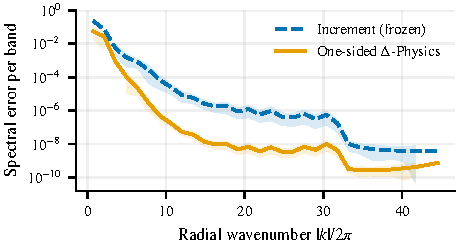
\includegraphics[width=\columnwidth]{fig4_spectral_error.pdf}
  \vspace{-1.8em}
  \caption{\textbf{Where the error is removed.} Per-band contribution to the spectral error, 2D Navier--Stokes, $\nu=2\nu_0$, step 50 (24 trajectories pooled across three seeds; band: $\pm$1 s.d.\ where positive).}
  \label{fig:spectral_error}
\end{figure}

\subsection{Why one-sided?}
\label{sec:why_one_sided}

To test the symmetric version, we applied the two-sided correction (without the indicator) across $\nu/\nu_0\in[0.5,2]$.
This is a separate diagnostic with a single seed on a $24\times24$ grid, not part of the three-seed $64\times64$ experiments (\cref{app:two_sided}).
Above $\nu_0$ it reproduces the monotone gains seen above.
Below $\nu_0$ it behaves as \cref{sec:one_sided} anticipates: at $\nu/\nu_0=0.5$ it improves step 1 by $10.53\%$, but turns negative by step 20 and reaches $-296.76\%$ at step 50.
Step-50 changes at $\nu/\nu_0=0.625$, $0.75$ and $0.875$ are $-52.29\%$, $-14.53\%$ and $-5.06\%$.
The energy-adding correction helps for a step and then degrades the rollout, so we switch it off. Because this is one seed at one resolution, the one-sided rule should be read as an empirical policy rather than a proven necessity.

\subsection{What do stronger alternatives cost?}
\label{sec:alternatives}

\begin{table*}[t]
\caption{\textbf{Original F-FNO: costlier alternatives.} 2D Navier--Stokes at $\nu/\nu_0=2$.
The first three rows reuse the same frozen checkpoint (24 training trajectories at $\nu_0$, 28,370 parameters);
the conditioned model is trained on five viscosities including every test value (28,386 parameters) and also
receives proportionally more optimizer updates, so it is an upper reference rather than an equal-budget competitor.
Inference: CPU wall-clock for 8 trajectories $\times$ 50 steps. Mean\,$\pm$\,s.d.\ over three seeds.}
\label{tab:alternatives}
\centering
\footnotesize
\setlength{\tabcolsep}{4pt}
\begin{tabular}{@{}l c c c c c c@{}}
\toprule
Method & \shortstack{Target-$\nu$\\data?} & \shortstack{Train\\traj.} & \shortstack{NN evals\\/ step} & \shortstack{Inference\\time (s)} & Avg-50 RelL2 & Step-50 RelL2 \\
\midrule
Frozen F-FNO & No & 24 & 1.00 & 7.53\std{0.83} & 0.2275\std{0.0275} & 0.4721\std{0.0680} \\
\quad + additive ($\Delta$-Physics) & No & 24 & 1.00 & 8.06\std{1.40} & 0.1791\std{0.0242} & 0.3682\std{0.0632} \\
\quad + input-Recast (iterative) & No & 24 & 8.81 & 70.08\std{8.50} & 0.1786\std{0.0242} & 0.3659\std{0.0630} \\
\midrule
Conditioned F-FNO (trained on all 5 $\nu$) & Yes & 120 & 1.00 & 7.38\std{0.32} & 0.0272\std{0.0008} & 0.0494\std{0.0011} \\
\bottomrule
\end{tabular}
\end{table*}


\Cref{tab:alternatives} places \method between two more expensive options at $\nu/\nu_0=2$ (also plotted in \cref{app:cost}).

\emph{More test-time compute.}
The Recast-style baseline converged on all 3,600 out-of-distribution trajectory-steps, with no NaN or Inf values, and needs on average 7.81 iterations, or 8.81 network evaluations per step.
It improves on \method by only $0.31\pm0.09\%$ in Avg-50 RelL2 and $0.62\pm0.10\%$ in Step-50 RelL2, while inference time rises from $8.06\pm1.40$\,s to $70.08\pm8.50$\,s.
In this setting, a single closed-form pass recovers nearly all of what the iteration achieves.

\emph{More training data.}
The conditioned F-FNO, trained with data at every test viscosity, is far more accurate: Avg-50 RelL2 $0.02716$ against $0.17915$ for \method.
It also uses five times as many trajectories (120 against 24) and 4.55$\times$ the optimiser time ($1275.70$ against $280.19$\,s per seed), with more gradient updates, so this is not an equal-budget comparison.
The conclusion is that \method is the option for when target-viscosity simulations do not exist, not a substitute for them when they do.

\subsection{Is the gain an artifact of an undertrained network?}
\label{sec:budget}

The 15-epoch reference models are small and far from converged: their Step-50 RelL2 is $0.4091$ even at $\nu_0$ (\cref{tab:main}).
To check that the correction is not just compensating for this, we retrained one seed for 75 epochs on the same data, which lowers the Step-50 error at $\nu_0$ from $0.37282$ to $0.09452$.
On this stronger model the gain at $\nu/\nu_0=2$ is \emph{larger}: Avg-50 RelL2 falls from $0.12423$ to $0.04634$ ($62.70\%$) and Step-50 RelL2 from $0.21283$ to $0.07819$ ($63.26\%$), compared with $23.94\%$ and $25.23\%$ for the 15-epoch model of the same seed (\cref{app:budget}).
This is a single-seed sensitivity check, but it suggests that the main results understate rather than overstate the effect.

%% ============================================================
\section{Related work}
\label{sec:related}

\textbf{Learning the parameter dependence from data.}
A common way to generalise across PDE parameters is to train on many of them: parameter- and time-scale conditioning \citep{gupta2023multiscale}, context-adapted dynamics models such as CoDA and GEPS \citep{kirchmeyer2022coda,koupai2024geps}, and multi-physics pretraining \citep{mccabe2024mpp,herde2024poseidon}.
\citet{zhu2023extrapolation} study operator extrapolation and improve it with physics-informed fine-tuning or sparse observations.
These approaches need training data or observations from the target regime; we assume only $\nu_0$ data and a known $\nu$.

\textbf{Reusing a frozen operator at test time.}
DISCO infers an evolution operator from trajectory context with a hypernetwork \citep{morel2025disco}, and Neural Operator Splitting searches a dictionary of learned operators to explain a short observed target trajectory \citep{serrano2026splitting}.
Both adapt without retraining but require target observations.
Closest to us are MD-PNOP and Equation Recast \citep{cheng2026mdpnop,cheng2026recast}, which derive parameter-induced operator changes from the governing equation, absorb them into effective source terms and solve the recast problem iteratively with a canonical operator, including zero-shot prediction in new parameter regimes.
Analytical, zero-shot parameter transfer is therefore not new in itself.
Our contribution is narrower: for an autoregressive time-stepper and a parameter that enters through a known linear dissipative term, the correction can be applied \emph{outside} the network in a single closed-form pass, and, empirically, it should be one-sided.
Our Recast-style adaptation (\cref{sec:alternatives}) suggests that, in this setting, the single pass loses less than 1\% accuracy relative to iterating while saving roughly 9$\times$ in network evaluations.

\textbf{Physics inside or around the learner.}
Physics-informed operators constrain training with equation residuals \citep{wang2021physicsdeeponet,li2024pino}, and hybrid solvers train learned corrections inside a numerical scheme \citep{um2020solverintheloop,kochkov2021mlcfd}.
Post-hoc corrections enforce invariants of a learned update \citep{mcgreivy2023invariants}; \citet{li2022chaotic} promote dissipativity in learned chaotic dynamics; and Deep-OSG builds the semigroup property into training \citep{chen2023deeposg}.
Exponential integrators use the exact propagator of the linear part of stiff problems \citep{hochbruck2010exponential}, and our correction borrows that structure; operator splitting composes the exact flows of the parts of a vector field \citep{strang1968construction,mclachlan2002splitting}.
\citet{gopakumar2026physical} build splitting into training, learning separate neural operators for the nonlinear physical operators while representing the linear operators with fixed finite-difference convolutions.
Unlike these methods, we leave training and the network untouched and use the propagator only to transfer an already trained model to a new parameter.

\textbf{Long-rollout accuracy.}
PDE-Refiner shows that low-amplitude, high-frequency content matters for long rollouts \citep{lippe2023pderefiner}, and APEBench argues that emulators should be judged on rollouts, not single steps \citep{koehler2024apebench}.
Our results fit this picture: the missing damping is small per step and concentrated at high frequencies, but it compounds over the rollout.

%% ============================================================
\section{Limitations}
\label{sec:limitations}

\begin{itemize}
  \setlength\itemsep{1pt}
  \item \textbf{One direction.} The method only handles shifts to higher viscosity. Lower viscosity, which is often the more interesting regime, falls back to the unchanged model, and the one-sided rule rests on a single-seed, low-resolution scan rather than on theory.
  \item \textbf{Known linear operator.} The correction requires the parameter to enter through a known linear dissipative operator; we validate only the periodic Laplacian. It does not model how viscosity changes the nonlinear dynamics.
  \item \textbf{Scale of the evidence.} Two PDEs on small grids ($64\times64$, 64 points), small training sets, viscosity ratios up to 2, and reference models trained for 15 epochs. The training-budget check and the two-sided scan each use one seed.
  \item \textbf{Baselines.} The Recast-style baseline is our own adaptation, not an official implementation. The conditioned baseline receives more optimizer updates. We have not yet compared against other one-evaluation ways of attaching the known physics (Lie or Strang splitting, an implicit post-step diffusion), which \cref{prop:local} suggests may be more accurate when the network is accurate, nor against few-shot fine-tuning.
  \item \textbf{No stability guarantee.} \Cref{prop:properties}(iii) characterises the correction alone, not the full nonlinear rollout.
\end{itemize}

%% ============================================================
\section{Conclusion}
\label{sec:conclusion}

When a physical parameter enters a PDE through a known linear dissipative term, a frozen neural time-stepper does not have to be retrained to follow it.
Adding the difference between the new and old diffusion propagators after each step, and only when it removes energy, makes the rollout error largely insensitive to a viscosity increase on the two PDEs we studied.
It does so at the cost of one FFT per step and with no target data.
Natural next steps are other known linear terms (hyperviscosity, damping, dispersion), non-periodic boundaries, comparison with operator-splitting variants, and combining the analytical correction with learned models of the nonlinear parameter dependence.

\section*{Impact Statement}
This work aims to make neural surrogates of physical systems cheaper to reuse when a physical parameter changes, which could reduce the simulation cost of design and what-if studies in engineering and science.
A risk is over-trust: a corrected surrogate can look physically plausible while still carrying large errors (\cref{tab:alternatives}), so outputs used for consequential decisions should be validated against trusted solvers.
We are not aware of other direct negative societal consequences.

\section*{Software and Data}
Code, frozen checkpoints, per-seed results and the scripts that generate every figure and table will be released (anonymised for review). All data are synthetic and produced by the included solvers.

\bibliography{../paper_draft/references,references_extra}
\bibliographystyle{icml2026}

%% ============================================================
\newpage
\appendix
\onecolumn

\section{Proofs}
\label{app:proofs}

\emph{(i)} At $\nu=\nu_0$ the indicator in \cref{eq:delta_physics} is zero, and in any case $S_\nu-S_{\nu_0}=0$, so the corrected step equals $\Phi_\theta$.

\emph{(ii)} With $\mathcal{N}=0$ and $\Phi_\theta=S_{\nu_0}$, for $\nu>\nu_0$ the corrected step is $S_{\nu_0}u+(S_\nu-S_{\nu_0})u=S_\nu u$ (\cref{eq:exact_linear}).

\emph{(iii)} Let $\mathcal{L}$ be self-adjoint and negative semidefinite with eigenvalues $\lambda_j\le0$ and orthonormal eigenfunctions $\phi_j$. Then $S_\nu-S_{\nu_0}$ has eigenvalues $e^{\nu\Delta t\lambda_j}-e^{\nu_0\Delta t\lambda_j}\le0$ for $\nu\ge\nu_0$, so $\langle u,(S_\nu-S_{\nu_0})u\rangle=\sum_j(e^{\nu\Delta t\lambda_j}-e^{\nu_0\Delta t\lambda_j})|\langle u,\phi_j\rangle|^2\le0$.
For the periodic Laplacian this is Parseval's identity with $\lambda=-|k|^2$:
\begin{equation*}
  \langle u,(S_\nu-S_{\nu_0})u\rangle=\sum_k\big(e^{-\nu|k|^2\Delta t}-e^{-\nu_0|k|^2\Delta t}\big)|\hat u(k)|^2\le0 .
\end{equation*}
For $\nu<\nu_0$ every multiplier changes sign, so the correction adds energy. The multipliers then lie in $[0,1)$, so $\|S_\nu-S_{\nu_0}\|\le1$: unlike the backward heat propagator $e^{-(\nu-\nu_0)|k|^2\Delta t}$, the correction is bounded. The one-sided rule therefore rests on the empirical scan of \cref{sec:why_one_sided}, not on this sign. The ratio $S_\nu(k)/S_{\nu_0}(k)=\exp[-(\nu-\nu_0)|k|^2\Delta t]$ decreases with $|k|$ for $\nu>\nu_0$, so relative attenuation is strongest at fine scales. The absolute multiplier in \cref{eq:fourier} is not monotone in $|k|$, since both exponentials vanish at sufficiently high frequency.

\textbf{Proof of \cref{prop:local}.}
On the spatially discretised state space all maps are smooth and $\mathcal{L}$ and $B$ are bounded, so we may expand in $h$ at fixed $u$; all terms below are evaluated at $u$. For a vector field $G$ with flow $\psi^h$, $\psi^h(u)=u+hG+\tfrac{h^2}{2}G'G+O(h^3)$. With $G=F_\nu=F_0+B$, where $F_0=\nu_0\mathcal{L}+\mathcal{N}$ and $F_\nu'=F_0'+B$,
\begin{equation*}
\varphi^h_\nu(u)=u+hF_0+hBu+\tfrac{h^2}{2}\big[F_0'F_0+F_0'Bu+BF_0+B^2u\big]+O(h^3).
\end{equation*}
The reference step is $\Phi_\theta(u)=\varphi^h_{\nu_0}(u)=u+hF_0+\tfrac{h^2}{2}F_0'F_0+O(h^3)$.

\emph{Additive.} Because $\mathcal{L}$ and $B$ commute, $S_\nu-S_{\nu_0}=e^{h\nu_0\mathcal{L}}(e^{hB}-I)=hB+\tfrac{h^2}{2}(2\nu_0\mathcal{L}B+B^2)+O(h^3)$. Subtracting $\Phi_{\mathrm{add}}(u)$ leaves $\tfrac{h^2}{2}[F_0'Bu+BF_0-2\nu_0\mathcal{L}Bu]$. With $F_0'=\nu_0\mathcal{L}+\mathcal{N}'$ and $BF_0=\nu_0\mathcal{L}Bu+B\mathcal{N}$, this equals $\tfrac{h^2}{2}[\mathcal{N}'(u)Bu+B\mathcal{N}(u)]$.

\emph{Lie.} $e^{hB}\Phi_\theta(u)=u+hF_0+hBu+\tfrac{h^2}{2}[F_0'F_0+2BF_0+B^2u]+O(h^3)$, so the difference is $\tfrac{h^2}{2}[F_0'Bu-BF_0]=\tfrac{h^2}{2}[\mathcal{N}'(u)Bu-B\mathcal{N}(u)]$; the $\nu_0\mathcal{L}B$ terms cancel because $\mathcal{L}$ and $B$ commute.

\emph{Strang.} $\Phi_{\mathrm{Str}}$ is the symmetric composition of the exact flows of $Bu$ and $F_0$, whose local error is $O(h^3)$ \citep{strang1968construction,mclachlan2002splitting}.

The constants in $O(h^3)$ grow with $\|B\|$, that is, with the shift and the resolution. A numerical check of all three expansions on a six-dimensional nonlinear system is part of the supplementary code (\texttt{check\_local\_error.py}).

\section{Experimental details}
\label{app:setup}

\textbf{Navier--Stokes.} $\partial_t\omega+\bm v\cdot\nabla\omega=\nu\Delta\omega+f$ on the periodic unit square, velocity recovered from the stream function, spectral derivatives with dealiasing of the advection term, RK4 with internal step $\delta t=0.005$; consecutive states given to the network are $\Delta t=0.05$ apart. Grid $64\times64$, $\nu_0=10^{-3}$, test ratios $\nu/\nu_0\in\{1,1.5,1.75,2\}$. Initial vorticity: a random periodic field with Fourier modes up to 4, normalised to unit standard deviation.
F-FNO: width 16, 8 retained modes per factorised Fourier branch, 8 residual layers, feed-forward expansion factor 4, Fourier weights shared across depth; inputs are the normalised vorticity and the two spatial coordinates; 28,370 parameters.

\textbf{Burgers.} $\partial_t u+u\,\partial_x u=\nu\,\partial_{xx}u$ on the periodic unit interval, spectral derivatives with dealiasing, RK4 with $\delta t=0.002$, network step $\Delta t=0.02$, 64 points, $\nu_0=10^{-2}$, test ratios $\nu/\nu_0\in\{1,1.25,1.5,1.75,2\}$. Initial conditions are random periodic fields. FNO1d: width 32, 16 retained modes, 4 Fourier layers with pointwise residual transforms. (F-FNO's dimension-wise factorisation degenerates to a single direction in 1D, so we use a standard FNO.)

\textbf{Data and training.} Per seed: 24 training and 6 validation trajectories at $\nu_0$, 20 transitions each (480 training pairs); 8 test trajectories per test viscosity; 50-step free-running rollouts without teacher forcing. Inputs and target increments are normalised with training-set statistics. MSE on normalised increments; Adam, learning rate $10^{-3}$, weight decay $10^{-6}$, batch size 32, 15 epochs, StepLR with factor 0.5 every 7 epochs; we keep the checkpoint with the lowest validation one-step RelL2. Seeds $\{0,1,2\}$. Experiments ran on CPU (four Torch threads); timings are hardware dependent.

\textbf{Metrics.} $\RelL=\|\hat u-u\|_2/\|u\|_2$; $\PSRE=\|P_{\hat u}-P_u\|_2/\|P_u\|_2$ with $P_u(k)=|\F[u](k)|^2$. Improvement $=100\times(E_\text{frozen}-E_\text{corrected})/E_\text{frozen}$, computed within each seed and then summarised across seeds.

\section{Recast-style baseline}
\label{app:recast}

Equation Recast and MD-PNOP were formulated for source-to-solution operators. Our model is a state-to-state time-stepper, so we use a dynamic, backward-Euler-style interpretation. Starting from $y^{(0)}=\Phi_\theta(u_t)$, we iterate the fixed-point map $G_\nu(y;u_t)=\Phi_\theta\big(u_t+\Delta t(\nu-\nu_0)\Delta y\big)$ with vector Aitken relaxation on the residual $r^{(k)}=G_\nu(y^{(k)};u_t)-y^{(k)}$, until the relative residual falls below $10^{-5}$ or 30 iterations are reached. Because $y$ enters the network's \emph{input}, every iteration needs a new network evaluation, which is why the baseline averages 8.81 evaluations per step. Adding the viscosity term outside the network instead, $y=\Phi_\theta(u_t)+\Delta t(\nu-\nu_0)\Delta y$, gives a different method, an implicit post-step diffusion $y=(I-\Delta t(\nu-\nu_0)\Delta)^{-1}\Phi_\theta(u_t)$ that needs one evaluation; it is among the variants not yet compared (\cref{sec:limitations}). At $\nu=\nu_0$ it reduces to one evaluation of the frozen model. \Cref{tab:recast_convergence} gives the convergence diagnostics.

\begin{table*}[!htbp]
\centering
\small
\resizebox{\textwidth}{!}{%
\begin{tabular}{rlccccc}
\toprule
$\nu/\nu_0$ & Mean iterations & P95 iterations & Max iterations & Mean NN evals / step & Non-converged steps & Inference time (s) \\
\midrule
1.0 & 0.00 & 0.0 & 0 & 1.00 & 0 & 7.32 $\pm$ 1.52 \\
1.5 & 5.86 & 6.0 & 6 & 6.86 & 0 & 48.22 $\pm$ 3.29 \\
1.75 & 6.41 & 7.0 & 8 & 7.41 & 0 & 61.20 $\pm$ 5.16 \\
2.0 & 7.81 & 8.0 & 9 & 8.81 & 0 & 70.08 $\pm$ 8.50 \\
\bottomrule
\end{tabular}%
}
\caption{Equation-Recast-style fixed-point diagnostics at tolerance $10^{-5}$ and at most 30 iterations. Counts pool three seeds, eight trajectories, and 50 physical steps per viscosity.}
\label{tab:recast_convergence}
\end{table*}


\section{Two-sided viscosity scan}
\label{app:two_sided}

\begin{figure}[h]
  \centering
  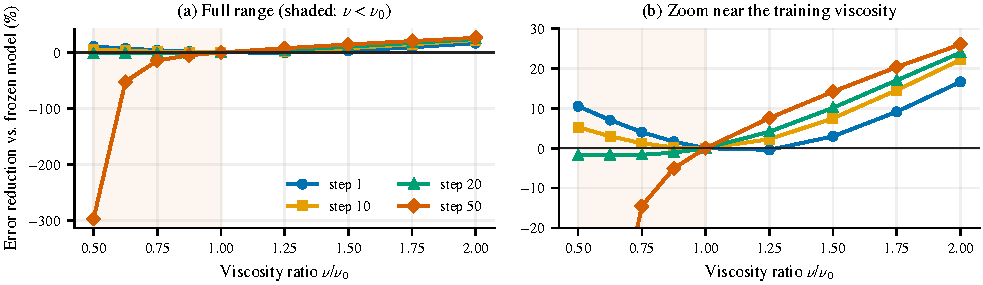
\includegraphics[width=\textwidth]{figA1_two_sided_scan.pdf}
  \caption{Two-sided correction (no indicator) on a separate $24\times24$ Navier--Stokes model, single seed. Improvement over the frozen network at steps 1--50. Above $\nu_0$ the gain grows with shift and horizon; below $\nu_0$ the correction helps early steps and then fails over long rollouts.}
  \label{fig:two_sided}
\end{figure}

\section{Accuracy against data and compute}
\label{app:cost}

The conditioned F-FNO uses the same width, modes, depth, optimiser, epochs and trajectories per viscosity as the single-viscosity model, and receives the standardised log-viscosity $q=(\log(\nu/\nu_0)-\mu_q)/\sigma_q$ as an extra constant input channel. It is trained jointly on $\nu/\nu_0\in\{1,1.25,1.5,1.75,2\}$, so every test viscosity is seen in training.

\begin{figure}[h]
  \centering
  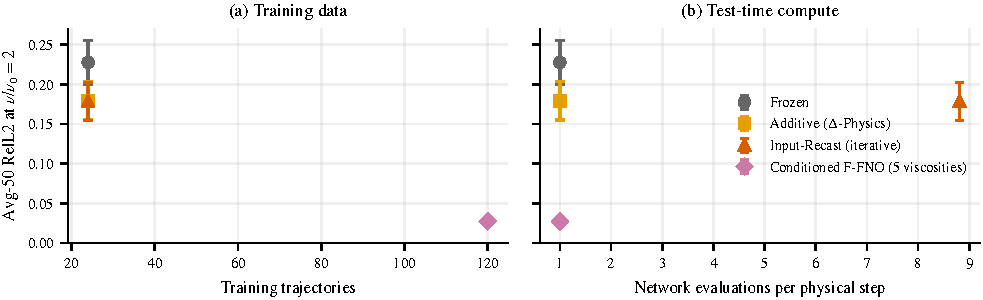
\includegraphics[width=\textwidth]{figA2_accuracy_cost.pdf}
  \caption{Average 50-step RelL2 at $\nu/\nu_0=2$ against training trajectories (a) and network evaluations per physical step (b), 2D Navier--Stokes; mean\,$\pm$\,s.d.\ over three seeds.}
  \label{fig:cost}
\end{figure}

\section{Sensitivity to the reference training budget}
\label{app:budget}

Same 24 training trajectories and seed 0; training extended from 15 to 75 epochs (the learning-rate schedule scales with the epoch budget). At $\nu=\nu_0$ the Step-50 RelL2 falls from $0.37282$ to $0.09452$, and \method preserves the stronger reference exactly. At $\nu/\nu_0=2$, the Avg-50 and final-step PSRE improvements are $83.81\%$ and $84.86\%$. Single seed; not part of the main three-seed comparison.

\begin{table}[h]
\caption{Zero-shot transfer with a 75-epoch reference F-FNO (seed 0). Gain: relative error reduction over the frozen network.}
\label{tab:training_budget}
\centering
\small
\begin{tabular}{c rrr rrr}
\toprule
& \multicolumn{3}{c}{Avg-50 RelL2} & \multicolumn{3}{c}{Step-50 RelL2} \\
\cmidrule(lr){2-4}\cmidrule(l){5-7}
$\nu/\nu_0$ & Frozen & $+\Delta$ & Gain (\%) & Frozen & $+\Delta$ & Gain (\%) \\
\midrule
1.00 & 0.05609 & 0.05609 & 0.00 & 0.09452 & 0.09452 & 0.00 \\
1.50 & 0.08028 & 0.04921 & 38.70 & 0.13899 & 0.08232 & 40.77 \\
1.75 & 0.10145 & 0.04753 & 53.15 & 0.17465 & 0.07985 & 54.28 \\
2.00 & 0.12423 & 0.04634 & 62.70 & 0.21283 & 0.07819 & 63.26 \\
\bottomrule
\end{tabular}
\end{table}

\section{Full-horizon tables}
\label{app:full_tables}

Complete Step-1/10/20/50 results behind the main figures; mean\,$\pm$\,s.d.\ over three seeds.

\input{../results/paper_assets/table_1_ns64_absolute.tex}
\input{../results/paper_assets/table_2_burgers_absolute.tex}

\end{document}
